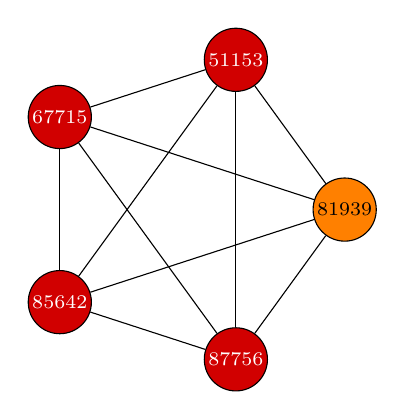
\begin{tikzpicture}
  \draw
    (0.000:2) node[fill=orange, text=black, font=\scriptsize, minimum size=4mm, inner sep=1pt, circle, draw] (81939){81939}
    (72.000:2) node[fill={rgb,140:red,255;green,0;blue,0}, font=\scriptsize, minimum size=3mm, inner sep=1pt, circle, draw, text=white] (51153){51153}
    (144.000:2) node[fill={rgb,140:red,255;green,0;blue,0}, font=\scriptsize, minimum size=3mm, inner sep=1pt, circle, draw, text=white] (67715){67715}
    (216.000:2) node[fill={rgb,140:red,255;green,0;blue,0}, font=\scriptsize, minimum size=3mm, inner sep=1pt, circle, draw, text=white] (85642){85642}
    (288.000:2) node[fill={rgb,140:red,255;green,0;blue,0}, font=\scriptsize, minimum size=3mm, inner sep=1pt, circle, draw, text=white] (87756){87756};
  \begin{scope}[-]
    \draw (51153) to (67715);
    \draw (51153) to (81939);
    \draw (51153) to (85642);
    \draw (51153) to (87756);
    \draw (67715) to (81939);
    \draw (67715) to (85642);
    \draw (67715) to (87756);
    \draw (81939) to (85642);
    \draw (81939) to (87756);
    \draw (85642) to (87756);
  \end{scope}
\end{tikzpicture}
